\section{Building \toolname}
\label{sec:plugin}

\toolname is a tool that collects fine-grained proof development data.
%without relying on a particular UI.
It is available on Github for Coq 8.10, with backported branches for
Coq 8.8 and Coq 8.9.\footnote{\url{http://github.com/uwplse/coq-change-analytics}}

\toolname works by instrumenting Coq to listen to user interaction.
Coq's interaction model (Section~\ref{sec:repl}) implements a REPL,
or Read Eval Print Loop: a loop that continually reads in messages
from the user, evaluates the statements those messages contain, 
and prints responses to the user.
All UIs for Coq, from the command line tool
\lstinline{coqtop}~\cite{coq-commands} to the IDEs CoqIDE~\cite{coqide} and
Proof General~\cite{Aspinall2000}, communicate with Coq through the REPL.
\toolname instruments the REPL to collect fine-grained data while remaining
decoupled from the UI.

Figure~\ref{fig:design} summarizes the design of \toolname.
\toolname is made of two parts: a client that the user installs,
and a web server that stores the data from multiple users.
The client instruments the REPL to record and log the data that the
user's UI sends to Coq (Section~\ref{sec:client}),
then sends this data to the server (Section~\ref{sec:server}),
which stores it for analysis.

The implementation effort for \toolname was modest, with just 412 LOC
of OCaml for the client and 178 LOC of Python for the server.%
\footnote{Counted using David M. Wheeler's SLOCCount.}
This modest effort was enough for us to collect 
(Section~\ref{sec:deployment}) and analyze 
(Sections~\ref{sec:q1} and~\ref{sec:q2}) data from hundreds
of interactive sessions.

\subsection{User-Coq Interaction}
\label{sec:repl}

% Is there a better source than this: http://paral-itp.lri.fr/papers/files/coq-workshop-paper.pdf
The \toolname client listens for messages that the user's UI
sends to Coq's REPL.
To provide a common API for different UIs, the implementation of
Coq's REPL is organized into an interactive state machine.
Each state can include tactics in Coq's tactic language Ltac or commands
in Coq's vernacular; both of these can reference terms in Coq's
specification language Gallina.
When a UI sends a message to Coq's REPL, the message contains a state
machine statement (a labeled transition) that instructs Coq to do one of three things:

\begin{enumerate}
\item \textit{Add}: produce a new state
\item \textit{Exec}: execute an existing state to receive a response
\item \textit{Cancel}: back up to an existing state
\end{enumerate}
Coq reacts accordingly, then returns an ID for the new state
that corresponds to the statement.

Taken together, these three statement types can be used
to reconstruct the proof engineer's behavior,
such as defining and redefining types, interactively constructing proofs,
and stepping up when the user hits a dead-end.

% Talia: Trying to get latex to display this in a reasonable place
\begin{figure}
  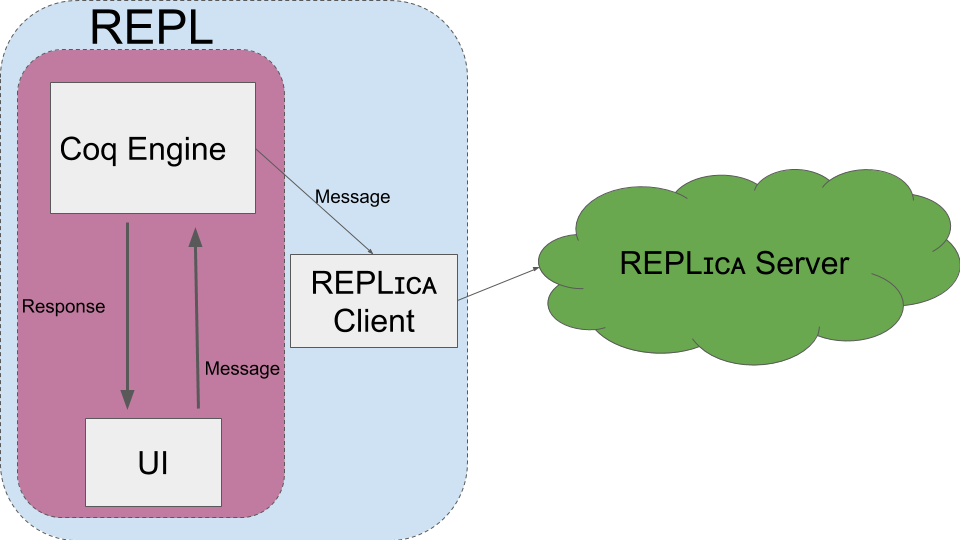
\includegraphics[width=0.8\columnwidth]{maintenance/fig/architecture.png}
\caption{\toolname design. The \toolname client listens to the REPL
and sends data to the \toolname server.}
\label{fig:design}
\end{figure}

\paragraph{From User Behavior to the State Machine}
When the user runs a command or tactic in Coq, the UI first adds
a new state corresponding to the command or tactic.
Adding a state to the state machine does not actually execute the
command or tactic;
to do that, the UI must execute the new state.
In other words, in state machine terms, each addition follows a transition,
but only returns the state number.
To get the state information, the UI must call \textit{Exec}.

Using this mechanism, the UI can group state machine statements and execute them
all at once. %, without interacting with the intermediate states.
For example, stepping down past 3 definitions at once in an IDE
manifests as 3 additions followed by a constant
number of executions, and successfully compiling a file manifests as 
many additions followed by a constant number of 
executions.\footnote{Some UIs send Coq multiple executions for each
group of additions.} 

When the user steps up in the UI, or attempts to run a tactic or command
that fails, the UI backs up to an existing state in the state machine.
Sending the state machine a cancellation statement is not the only way to back up to
an existing state; cancellations can also take the form of state machine
\textit{additions} of \lstinline{Cancel} or \lstinline{BackTo} commands
in Coq's vernacular. In either form, cancellations take a state ID
as an argument to specify the state to back up to.
%% Trying a statement that fails manifests as a cancellation,
%% and stepping up in an IDE manifests as a cancellation
%% followed by an IDE signature;
%% Section~\ref{sec:discussion} discusses distinguishing between these.

\paragraph{An Example: Defining and Extending an Inductive Type}
To see how user behavior corresponds to state machine statements,
consider an example from User 1, Session 41, simplified for readability.
In this session, User 1 stepped past
the definition of an inductive type \lstinline{Alpha}. Later, User 1
stepped above \lstinline{Alpha}, imported list notations,
then stepped down to add a new constructor to \lstinline{Alpha}
using those notations.

When User 1 first stepped down below \lstinline{Alpha},
Coq received a state machine addition (denoted
\lstinline{Add}, following SerAPI~\cite{GallegoArias2016SerAPI})
of this definition (again simplified for readability):

\begin{lstlisting}
  (Add () "Inductive Alpha : $\ldots$ := $\ldots$")
\end{lstlisting}
at the state ID \lstinline{1}, producing state ID \lstinline{2}.
Since User 1 stepped down a single step, Coq also received
an execution (denoted \lstinline{Exec}) of the new state:

\begin{lstlisting}
  (Exec 2)
\end{lstlisting}
which did not produce a state with a new state ID, since only additions
produce states, and only states have state IDs.
When User 1 stepped up to above the definition of \lstinline{Alpha},
Coq received a cancellation (denoted \lstinline{Cancel}):

\begin{lstlisting}
  (Cancel 1)
\end{lstlisting}
taking the state machine to before the definition of \lstinline{Alpha}.
When User 1 added the import, Coq
received an addition at state ID \lstinline{1}, producing state ID
\lstinline{3}, followed by an execution:

\begin{lstlisting}
  (Add () "Import Coq.Lists.List.ListNotations. ")
  (Exec 3)
\end{lstlisting}
Finally, when User 1 added the new constructor to \lstinline{Alpha}
and stepped down past it,
Coq received an addition of \lstinline{Alpha} with the new
constructor at state ID  \lstinline{3} producing state ID \lstinline{4}, followed by an execution:

\begin{lstlisting}
  (Add () "Inductive Alpha : $\ldots$ := $\ldots$
             | alpha_rec_mt : $\ldots$")
  (Exec 4)
\end{lstlisting}

The data that \toolname received provided us with enough
information to visualize these changes as a sequence of
diffs for later analysis (Section~\ref{sec:q2}).
As a consequence, we were able to find this pattern of development
of incrementally extending inductive types for four of our users
(Section~\ref{sec:pat1}).

\subsection{User-Client Interaction}
\label{sec:client}

The \toolname client records all of the additions, executions,
and cancellations that the proof engineer's UI or compiler sends.
To use it, the proof engineer installs the client,
then adds a line to the Coq requirements file~\cite{coqrc} so that
Coq always loads it.
On the first build, \toolname asks the proof engineer for consent and
for demographic information for the study.
From then on, the proof engineer uses Coq normally.

The implementation of the client is a Coq plugin.
Coq's plugin system makes it possible to extend
Coq without compromising trust in the Coq core.
\toolname does not include new commands or tactics; it simply attaches
to Coq's REPL and listens for messages that the proof engineer sends to Coq.

The hooks in the plugin API that allow plugins to listen to the REPL
were not initially present in Coq;
we worked with one of the Coq developers
to add this to Coq 8.10.\footnote{\url{http://github.com/coq/coq/pull/8768}}
We also developed backported branches of Coq 8.8 and 8.9 that include
this API, so that users whose projects depended on those
versions of Coq could participate in our study. This API is now available in all
versions of Coq going forward. %so that other study and plugin authors
%can use it.

\subsection{Client-Server Interaction}
\label{sec:server}

To record a history of user behavior,
the \toolname client sends a record of each state machine addition,
execution, and cancellation to the \toolname server.
The server then collects this data into a format suitable for analysis.

The message that the client sends to the server includes both the
state machine statement and additional metadata.
\iffalse
For example, a full message to the server for the simplified example
from Section~\ref{sec:repl} looks like this:

\begin{lstlisting}
((time 1567665712.25)
 (id 2)
 (user 1)
 (session-module gamma_completeness_implies_ec_assoc)
 (session 1567665710.63)
 (Control
   (Add () "Inductive Alpha : $\ldots$ := $\ldots$")))
\end{lstlisting}
where \lstinline{time} is the time the state change occurred,
\lstinline{id} is the state of the addition,
\lstinline{user} is the user ID,
\lstinline{session-module} is the Coq module in which the statements
were executed,
\lstinline{session} is the start time of the session,
and the body of the messages beginning with \lstinline{Control}
is the addition to the state machine.
%\todo{what do we do about our off-by-one errors?}
\fi

\begin{figure*} % Talia: For good table placement
\begin{minipage}{0.67\textwidth}
\small
\centering
\begin{tabular}{ |l|l|l|l|l|l|l| }
 \hline
  \textbf{User} & \textbf{Years} & \textbf{Expertise} & \textbf{Purpose} & \textbf{Frequency} & \textbf{UI} & \textbf{Version} \\
\hline
  \textbf{0} & 2-4 & $\circ$ $\circ$ $\circ$ $\circ$ $\circ$ & Verification & Daily & Proof General & Master \\
  \textbf{1} & 2-4 & $\circ$ $\circ$ $\circ$ & Mathematics & Monthly & Proof General & 8.10 \\
  \textbf{2} & > 4 & $\circ$ $\circ$ $\circ$ $\circ$ & Verification & Daily & Proof General & 8.10 \\
  \textbf{3} & > 4 & $\circ$ $\circ$ $\circ$ $\circ$ $\circ$ & Verification & Weekly & Proof General & Master \\
  \textbf{4} & > 4 & $\circ$ $\circ$ $\circ$ $\circ$ & Verification & Daily & coqtop & Master \\
  \textbf{5} & 2-4 & $\circ$ $\circ$ $\circ$ & Verification & Monthly & Custom & 8.10 \\
  \textbf{6} & 2-4 & $\circ$ $\circ$ $\circ$ $\circ$ & Mathematics & Daily & Proof General & Master \\
  \textbf{7} & 2-4 & $\circ$ $\circ$ $\circ$ $\circ$ & Mathematics & Weekly & Proof General & 8.10 \\
  \textbf{8} & > 4 & $\circ$ $\circ$ $\circ$ $\circ$ $\circ$ & Verification & Daily & Proof General & 8.8 \\
  \textbf{9} & > 4 & $\circ$ $\circ$ $\circ$ $\circ$ $\circ$ & Verification & Monthly & Proof General & 8.9 \\
  \textbf{10} & > 4 & $\circ$ $\circ$ $\circ$ & Verification & Daily & Proof General & 8.8 \\
  \textbf{11} & > 4 & $\circ$ $\circ$ $\circ$ & Mathematics & Daily & Proof General & 8.9 \\
\hline
\end{tabular}
\caption{User profiles of Coq development
background: experience in years, self-assessed expertise (beginner, novice, intermediate, knowledgeable, or expert, represented by circles), purpose of use, frequency of use, UI, and current version.}
\label{tab:users}
\end{minipage}
\hfill
\begin{minipage}{0.31\textwidth}
\small
\centering
\begin{tabular}{ |l|l|l|l| }
 \hline
  \textbf{User} & \textbf{Total} & \textbf{Interactive} & \textbf{Proof}\\
\hline
  \textbf{0} & 6 &  0 & 0 \\
  \textbf{1} & 42 & 10 & 4 \\
  \textbf{2} & 7 & 3 & 0 \\
  \textbf{3} & 11495 & 101 & 8 \\
  \textbf{4} & 1 & 0 & 0 \\
  \textbf{5} & 41 & 15 & 16 \\
  \textbf{6} & 1 & 0 & 0 \\
  \textbf{7} & 229 & 183 & 241 \\
  \textbf{8} & 162 & 27 & 10 \\
  \textbf{9} & 5 & 0 & 0 \\
  \textbf{10} & 23 & 15 & 0 \\
  \textbf{11} & 17 & 8 & 0 \\
\hline
\end{tabular}
\caption{Number of total sessions, interactive sessions,
  and interactive proof subsessions per user.}
\label{tab:sessions}
\end{minipage}
\end{figure*}

\paragraph{Metadata for Two Challenges}
The metadata beyond the state ID and the state machine
statement exists to handle two challenges:
The first challenge is that state machine interactions alone
are not enough to reconstruct a per-user history,
nor to group the user's interaction into discrete sessions
for a particular project or module.
The second challenge is that the network can be slow or unreliable at times,
causing messages to be received by the server out of order,
and slowing down the UI if not handled properly.

To handle the first challenge, \toolname labels each message with
a module name, user ID, and session ID.
The module name comes from the Coq plugin API.
The user ID is generated by the server and stored on the user's machine.
\iffalse
When a user builds the client for the first time, it contacts the server
and receives a unique user ID, which is stored locally on the
user's machine.
\fi
The session ID, in contrast, is generated by the client:
When the user loads the client, upon opening any new file,
the client records the start time of the session.
This start time is then used to identify the session.

To handle the second challenge, \toolname{} labels each message
with two pieces of metadata: the time at which the state machine message was sent to Coq (to order messages)
and the state ID (to detect missing states).
TCP alone is not enough to address these issues since each invocation
of the plugin creates a separate network stream
(so the server may receive messages out of order),
and since the user can disable the plugin
(so the client may never send some 
messages).\footnote{The consent form allowed users to temporarily disable
the plugin if necessary, as long as they informed us of this.} 
In addition to this metadata,
%instead of sending messages as soon as they are ready,
\toolname{} sends messages in batches.
If the network is not available, \toolname{} logs messages locally,
then sends those logs to the server the next time
the network is available.
